\documentclass[aspectratio=169, 10pt]{beamer}

\usetheme{Madrid}
\usecolortheme{default}
\definecolor{ATLASblue}{RGB}{0, 51, 102}
\definecolor{ATLASgold}{RGB}{200, 160, 0}
\setbeamercolor{structure}{fg=ATLASblue}
\setbeamercolor{frametitle}{bg=ATLASblue, fg=white}
\setbeamercolor{title}{bg=ATLASblue, fg=white}
\setbeamercolor{block title}{bg=ATLASblue!80, fg=white}
\setbeamercolor{block body}{bg=ATLASblue!8}
\setbeamercolor{alerted text}{fg=ATLASgold}
\setbeamerfont{frametitle}{size=\large, series=\bfseries}

\usepackage[utf8]{inputenc}
\usepackage[T1]{fontenc}
\usepackage[italian]{babel}
\usepackage{amsmath}
\usepackage{booktabs}
\usepackage{multirow}
\usepackage{tikz}
\usetikzlibrary{arrows.meta, positioning, shapes.geometric}

\title[GN2 Jet Flavour Tagging]{%
    \textbf{Jet Flavour Tagging con Transformer (GN2)}\\
    \small Implementazione in PyTorch}
\subtitle{ATLAS Collaboration --- \textit{Nat.\ Commun.}\ \textbf{17}, 541 (2026)}
\author{Luca Nasini (656244)}
\date{\today}

\setbeamertemplate{footline}{
    \leavevmode\hbox{%
        \begin{beamercolorbox}[wd=.5\paperwidth,ht=2.25ex,dp=1ex,center]{author in head/foot}
            \usebeamerfont{author in head/foot}\insertshorttitle
        \end{beamercolorbox}
        \begin{beamercolorbox}[wd=.5\paperwidth,ht=2.25ex,dp=1ex,right]{date in head/foot}
            \usebeamerfont{date in head/foot}\insertframenumber{}/\inserttotalframenumber\hspace*{2ex}
        \end{beamercolorbox}}
}
\setbeamertemplate{navigation symbols}{}

\begin{document}

\begin{frame}
    \titlepage
    \vspace{1mm}
    \begin{center}
        \textbf{Obiettivo:} addestrare un transformer a classificare i jet di
        collisioni $pp$ come $b$, $c$, $\tau$ o \textit{light} a partire
        dalle tracce di particelle cariche associate al jet
    \end{center}
\end{frame}


\begin{frame}{Perché il Jet Flavour Tagging?}
    \begin{columns}[T]
        \begin{column}{0.48\textwidth}
            \begin{block}{Contesto fisico}
                \begin{itemize}
                    \item I jet adronici sono gli oggetti più abbondanti nelle collisioni $pp$ all'LHC
                    \item Identificare il sapore del quark d'origine è fondamentale per studiare il Modello Standard
                \end{itemize}
            \end{block}
            \begin{block}{Quattro classi}
                \centering\vspace{2mm}
                \begin{tabular}{cl}
                    \toprule
                    Classe & Descrizione \\
                    \midrule
                    $b$-jet     & contiene un adrone-$b$ \\
                    $c$-jet     & contiene un adrone-$c$ \\
                    $\tau$-jet  & decadimento adronico di $\tau$ \\
                    light-jet   & quark leggero o gluone \\
                    \bottomrule
                \end{tabular}
                \vspace{2mm}
            \end{block}
        \end{column}
        \begin{column}{0.48\textwidth}
            \begin{block}{Approcci al flavour tagging}
                \textbf{Pipeline tradizionale (a due stadi):}
                \begin{enumerate}
                    \item Algoritmi di basso livello $\rightarrow$ ricostruiscono i
                          vertici spostati
                    \item Classificatore multivariato ad alto livello
                          (e.g.\ DL1d) $\rightarrow$ combina gli output
                \end{enumerate}
                \vspace{4pt}
                \textbf{GN2:} un unico transformer \textit{end-to-end}
            \end{block}
            \begin{alertblock}{Confronto: DL1d vs. GN2}
                Miglioramento di un fattore $1.5-4$
            \end{alertblock}
        \end{column}
    \end{columns}
\end{frame}


\begin{frame}{Preprocessing (\texttt{preprocess.py})}
    \begin{columns}[T]
        \begin{column}{0.48\textwidth}
            \begin{block}{Dati di input (HDF5, simulazione MC $t\bar{t}$)}
                \begin{itemize}
                    \item \textbf{5.6 milioni} di jet totali, 4 categorie di sapore
                    \item \textbf{Livello jet:} $p_T$, $\eta$
                    \item \textbf{Livello traccia:} $d_0$, $z_0$, significanze, variabili angolari; flag \texttt{valid} per le tracce utilizzabili
                \end{itemize}
            \end{block}
            \begin{block}{Selezione cinematica}
                \centering
                $20 < p_T < 250$~GeV \quad\&\quad $|\eta| < 2.5$
            \end{block}
        \end{column}
        \begin{column}{0.48\textwidth}
            \begin{block}{Normalizzazione senza data leakage}
                Media e deviazione standard calcolate \textbf{esclusivamente sul training set}\\
                Statistiche salvate in \texttt{norm\_stats.json}
            \end{block}
            \begin{block}{Splitting (per indice casuale)}
                \centering
                Train 70\% \;/\; Validation 20\% \;/\; Test 10\%\\
                Indici salvati in \texttt{XXX\_indices.npy}
            \end{block}
        \end{column}
    \end{columns}
    \begin{center}
        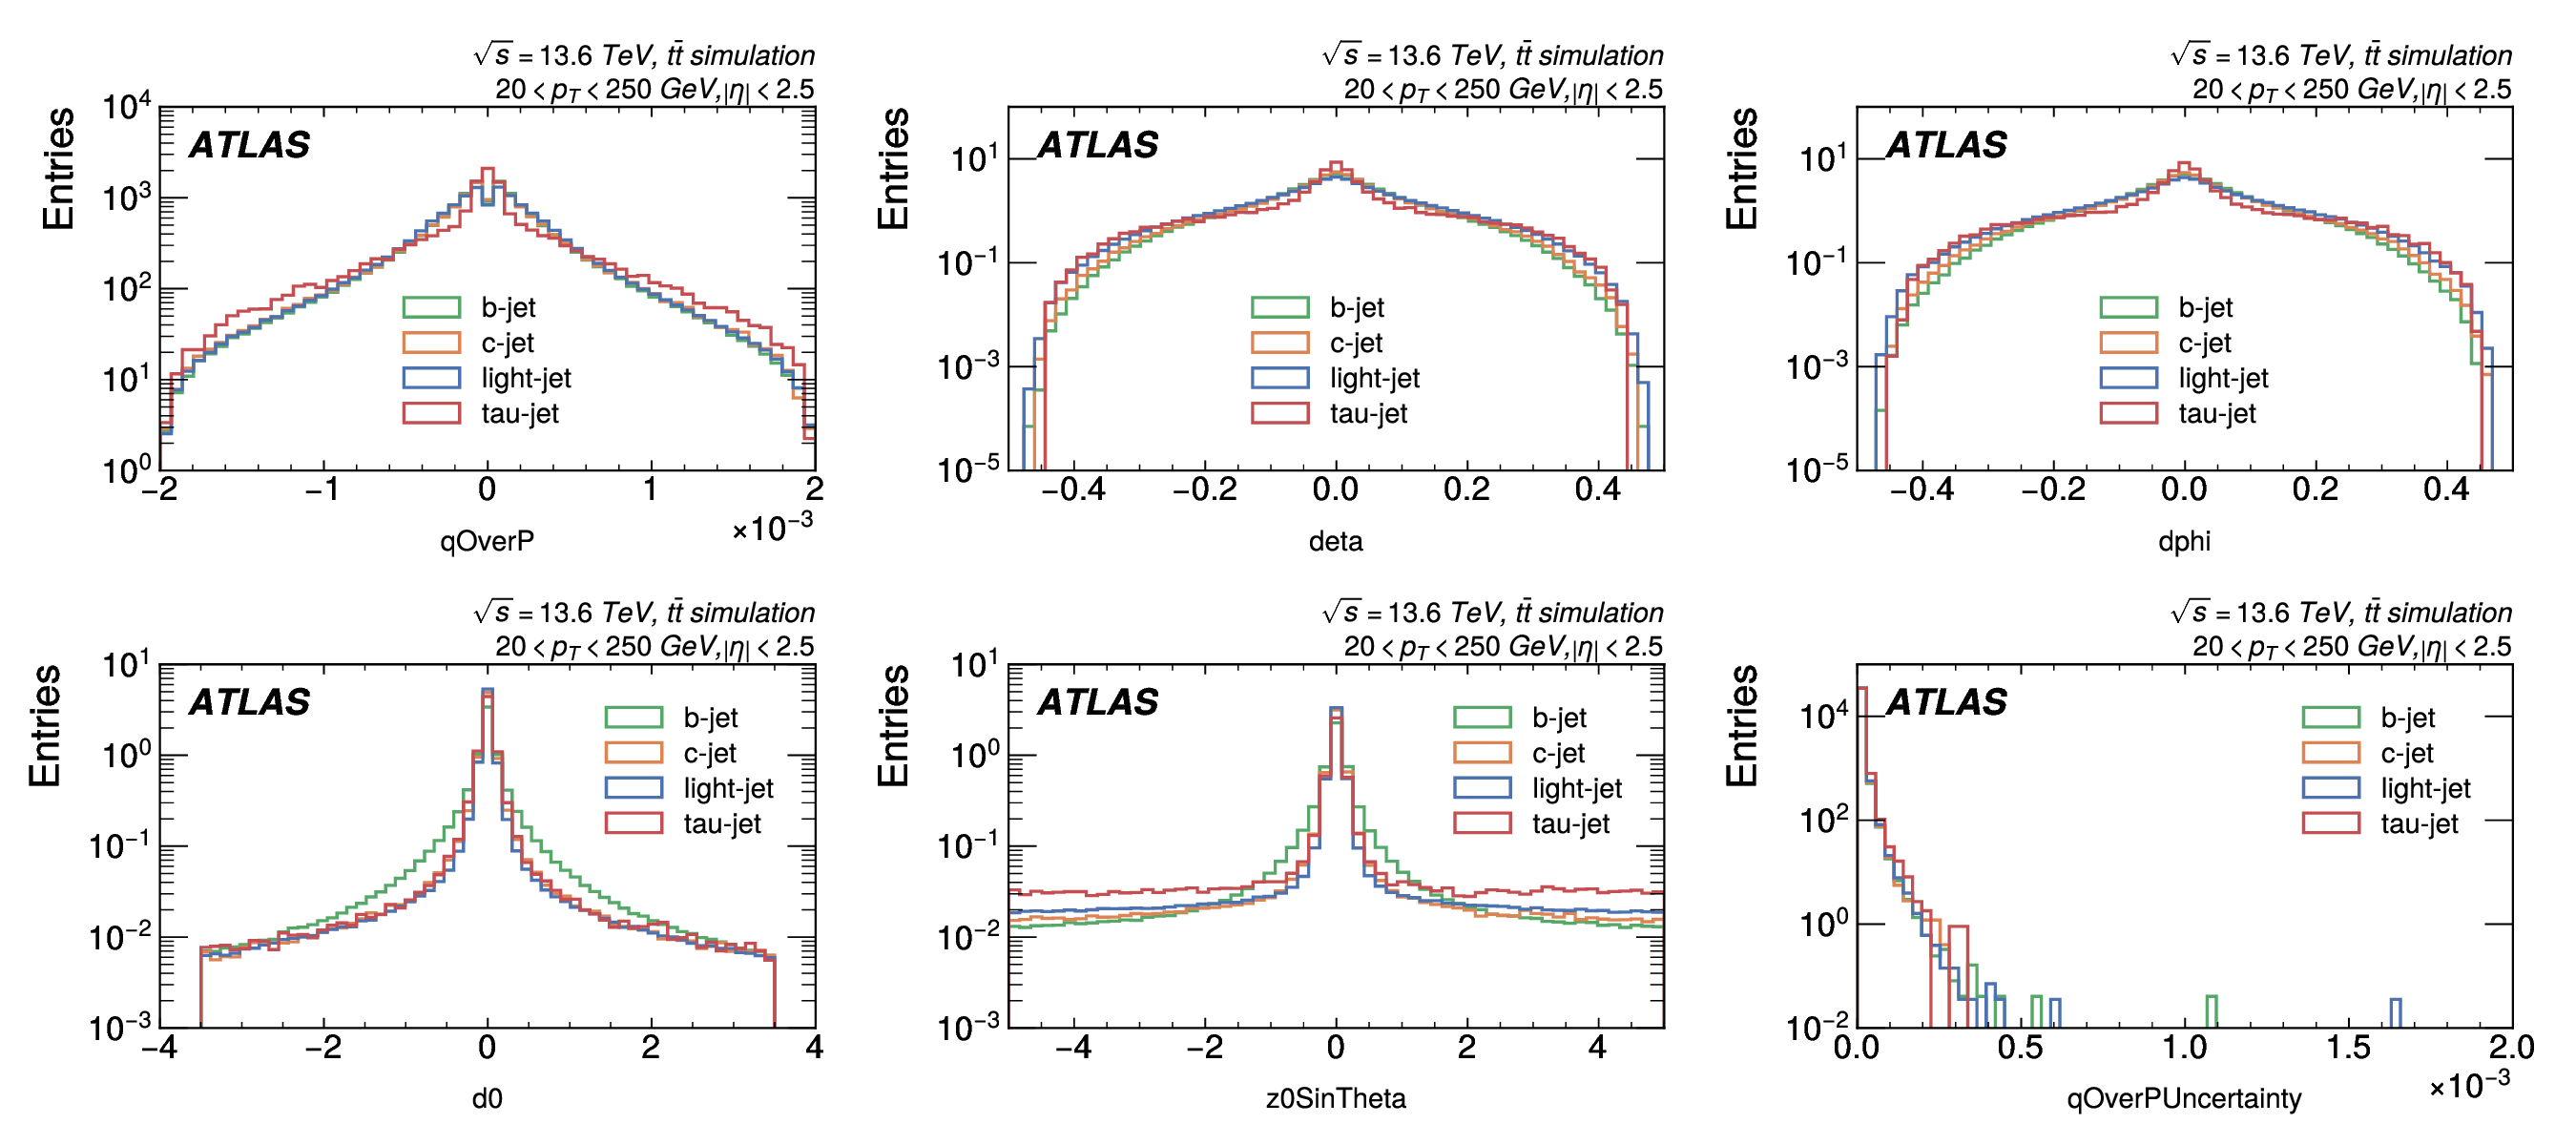
\includegraphics[width=0.82\linewidth]{../../results/data_statistics/track_variables_page1.png}
    \end{center}
\end{frame}


\begin{frame}{Caricamento Efficiente dei Dati (\texttt{dataset.py})}
    \begin{columns}[T]
        \begin{column}{0.48\textwidth}
            \begin{block}{Tre componenti principali}
                \begin{itemize}
                    \item \textbf{\texttt{GN2Dataset}}: padding/crop a 40 tracce, normalizzazione, lock su HDF5 per evitare race condition
                    \item \textbf{\texttt{\_IndexDataset}}: restituisce solo gli indici dei campioni $\to$ garantendo accessi ordinati e contigui su disco
                    \item \textbf{\texttt{\_BatchCollator}}: ordina i jet in un batch per letture HDF5 contigue $\to$ riducendo l'overhead di I/O
                \end{itemize}
            \end{block}
        \end{column}
        \begin{column}{0.48\textwidth}
            \begin{block}{Gestione del padding}
                Ogni jet ha un numero variabile di tracce. Le posizioni non valide vengono:
                \begin{itemize}
                    \item azzerate con maschera booleana durante la lettura
                    \item escluse dall'attenzione del transformer tramite la stessa maschera
                \end{itemize}
            \end{block}
        \end{column}
    \end{columns}
    \begin{alertblock}{Risultato}
        \texttt{gn2\_dataloader} costruisce un \texttt{DataLoader} PyTorch con batch ordinati e ottimizzati per il training
    \end{alertblock}
\end{frame}


\begin{frame}{Architettura del Modello (\texttt{model.py})}
    \begin{columns}[T]
        \begin{column}{0.26\textwidth}
            \begin{tikzpicture}[
                box/.style={rectangle,
                rounded corners=3pt,
                draw=ATLASblue,
                fill=ATLASblue!12,
                minimum width=3.6cm,
                minimum height=0.65cm,
                font=\small,
                align=center},
                arr/.style={-{Stealth[length=4pt]}, ATLASblue, thick},
                node distance=0.38cm]
                \node[box] (inp) {Var. jet $\oplus$ Var. traccia\\
                                  \small $(B,\,F_j{+}F_t,\,T)$};
                \node[box, below=of inp] (init)
                    {\textbf{Inizializzatore per-traccia}\\
                     \small MLP 2 strati $\to$ dim.\ 64};
                \node[box, below=of init] (tf)
                    {\textbf{Encoder Transformer}\\
                     \small 4 strati, 8 teste,\\emb=64, ff=256};
                \node[box, below=of tf] (pool)
                    {\textbf{Attention Pooling}\\
                     \small $\sum_i w_i \mathbf{e}_i \to (B,128)$};
                \node[box, below=of pool] (head)
                    {\textbf{Testa di Classificazione}\\
                     \small MLP: $128\!\to\!64\!\to\!32\!\to\!4$};
                \node[box, below=of head, fill=ATLASgold!20,
                      draw=ATLASgold] (out)
                    {$(p_b,\;p_c,\;p_u,\;p_\tau)$};
                \draw[arr] (inp)--(init);
                \draw[arr] (init)--(tf);
                \draw[arr] (tf)--(pool);
                \draw[arr] (pool)--(head);
                \draw[arr] (head)--(out);
            \end{tikzpicture}
        \end{column}
        \begin{column}{0.7\textwidth}
            \begin{block}{1 - Inizializzatore per-traccia}
                Concatenazione di tutte le variabili (jet + track).
                Un MLP a due strati mappa il vettore combinato in uno spazio di dimensione 64.
            \end{block}
            \begin{block}{2 - Encoder Transformer (Pre-LayerNorm)}
                Per ogni layer $\ell$:
                \(
                    \mathbf{x}' = \mathbf{x} + \mathrm{MHA}(\mathrm{LN}(\mathbf{x})),
                    \quad
                    \mathbf{x}'' = \mathbf{x}' + \mathrm{FFN}(\mathrm{LN}(\mathbf{x}'))
                \)
            \end{block}
            \begin{block}{3 - Attention Pooling}
                \[
                    w_i = \mathrm{softmax}(\mathbf{q}^\top \mathbf{e}_i)
                    \quad \to \quad
                    \mathbf{z} = \sum_i w_i \mathbf{e}_i
                \]
                Jet completamente mascherati ricevono pesi uniformi.
            \end{block}
            \begin{alertblock}{}
                \centering
                $\Rightarrow \quad \sim$\textbf{230\,000} parametri addestrabili
            \end{alertblock}
        \end{column}
    \end{columns}
\end{frame}


\begin{frame}{Addestramento (\texttt{train.py})}
    \begin{columns}[T]
        \begin{column}{0.60\textwidth}
            \begin{block}{Loss, ottimizzatore e learning rate schedule}
                \textbf{Loss:} cross-entropy a 4 classi (\texttt{ignore\_index=-1})
                \textbf{Ottimizzatore:} AdamW, weight decay $\lambda = 10^{-5}$
                \begin{enumerate}
                    \item Warmup lineare: $10^{-7} \to 5\times10^{-4}$ (primo 1\% degli step)
                    \item Cosine annealing: $5\times10^{-4} \to 10^{-5}$
                \end{enumerate}
            \end{block}
            \begin{center}
                \begin{figure}
                    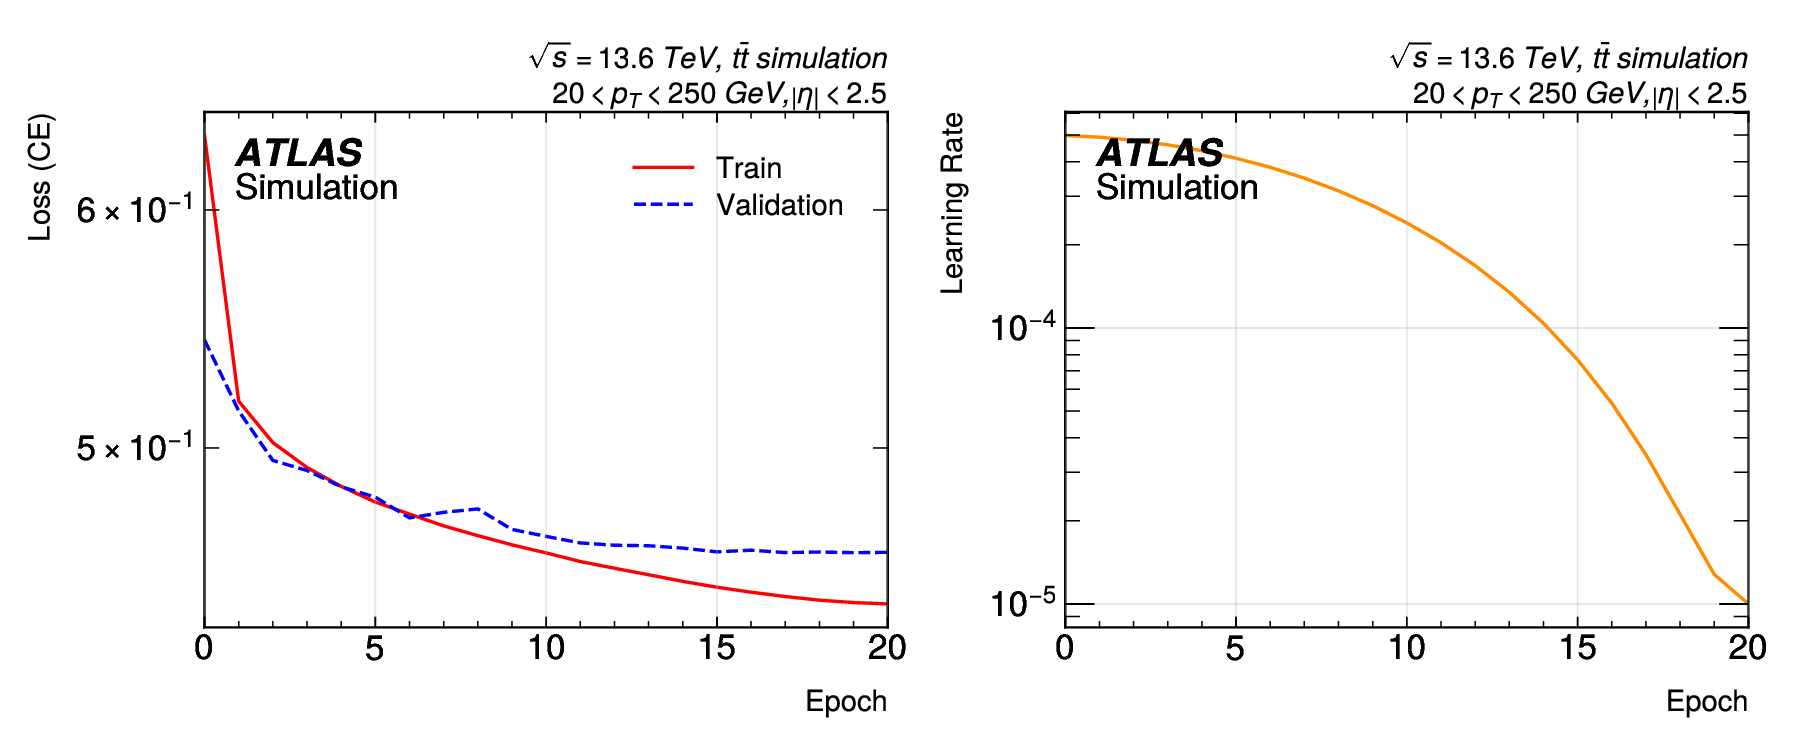
\includegraphics[width=0.98\linewidth]{../../results/learning_curves.png}
                \end{figure}
            \end{center}
        \end{column}
        \begin{column}{0.36\textwidth}
            \begin{block}{Iperparametri principali}
                \centering\vspace{2pt}
                \begin{tabular}{lc}
                    \toprule
                    Iperparametro   & Valore \\
                    \midrule
                    Epoche          & 21 \\
                    Batch size      & 2048 \\
                    Max tracce      & 40 \\
                    Attivazione     & ReLU \\
                    Dropout         & No \\
                    Grad. clipping  & $\|\nabla\| \le 1.0$ \\
                    \midrule
                    Dispositivo     & GPU Tesla T4 \\
                    Tempo training  & $\sim$17 ore \\
                    \bottomrule
                \end{tabular}
                \vspace{2pt}
            \end{block}
        \end{column}
    \end{columns}
\end{frame}


\begin{frame}{Discriminanti di Tagging e Curve ROC (\texttt{evaluate.py})}
    \begin{columns}[T]
        \begin{column}{0.48\textwidth}
            \begin{block}{Discriminante $b$-tagging ($D_b$)}
                \[
                    D_b = \log\!\left(\frac{p_b}{f_c\,p_c + f_\tau\,p_\tau
                    + (1{-}f_c{-}f_\tau)\,p_u}\right)
                \]
                Parametri ATLAS: $f_c = 0.20$, $f_\tau = 0.05$
            \end{block}
        \end{column}
        \begin{column}{0.48\textwidth}
            \begin{block}{Discriminante $c$-tagging ($D_c$)}
                \[
                    D_c = \log\!\left(\frac{p_c}{f_b\,p_b + f_\tau\,p_\tau
                    + (1{-}f_b{-}f_\tau)\,p_u}\right)
                \]
                Parametri ATLAS: $f_b = 0.30$, $f_\tau = 0.01$
            \end{block}
        \end{column}
    \end{columns}
    \vspace{0.5cm}
    \begin{columns}[T]
        \begin{column}{0.53\textwidth}
            \begin{block}{Curve ROC: rigetto vs. efficienza}
                Per ogni classe di fondo $k$ e soglia $\theta$:
                \[
                    R_k(\theta) =
                    \frac{|\text{fondo}_k|}{|\{D>\theta\}\cap\text{fondo}_k|}
                \]
                Rigetto maggiore a pari efficienza $=$ tagger migliore
            \end{block}
        \end{column}
        \begin{column}{0.43\textwidth}
            \begin{block}{Output prodotti}
                \begin{itemize}
                    \item \texttt{metrics.json}
                    \item \texttt{confusion\_matrix.pdf}
                    \item \texttt{score\_distributions.pdf}
                    \item \texttt{roc\_db.pdf}, \texttt{roc\_dc.pdf}
                \end{itemize}
            \end{block}
        \end{column}
    \end{columns}
\end{frame}


\begin{frame}{Distribuzioni degli Score e Matrice di Confusione}
    \begin{columns}[T]
        \begin{column}{0.50\textwidth}
            \begin{center}
                \begin{figure}
                    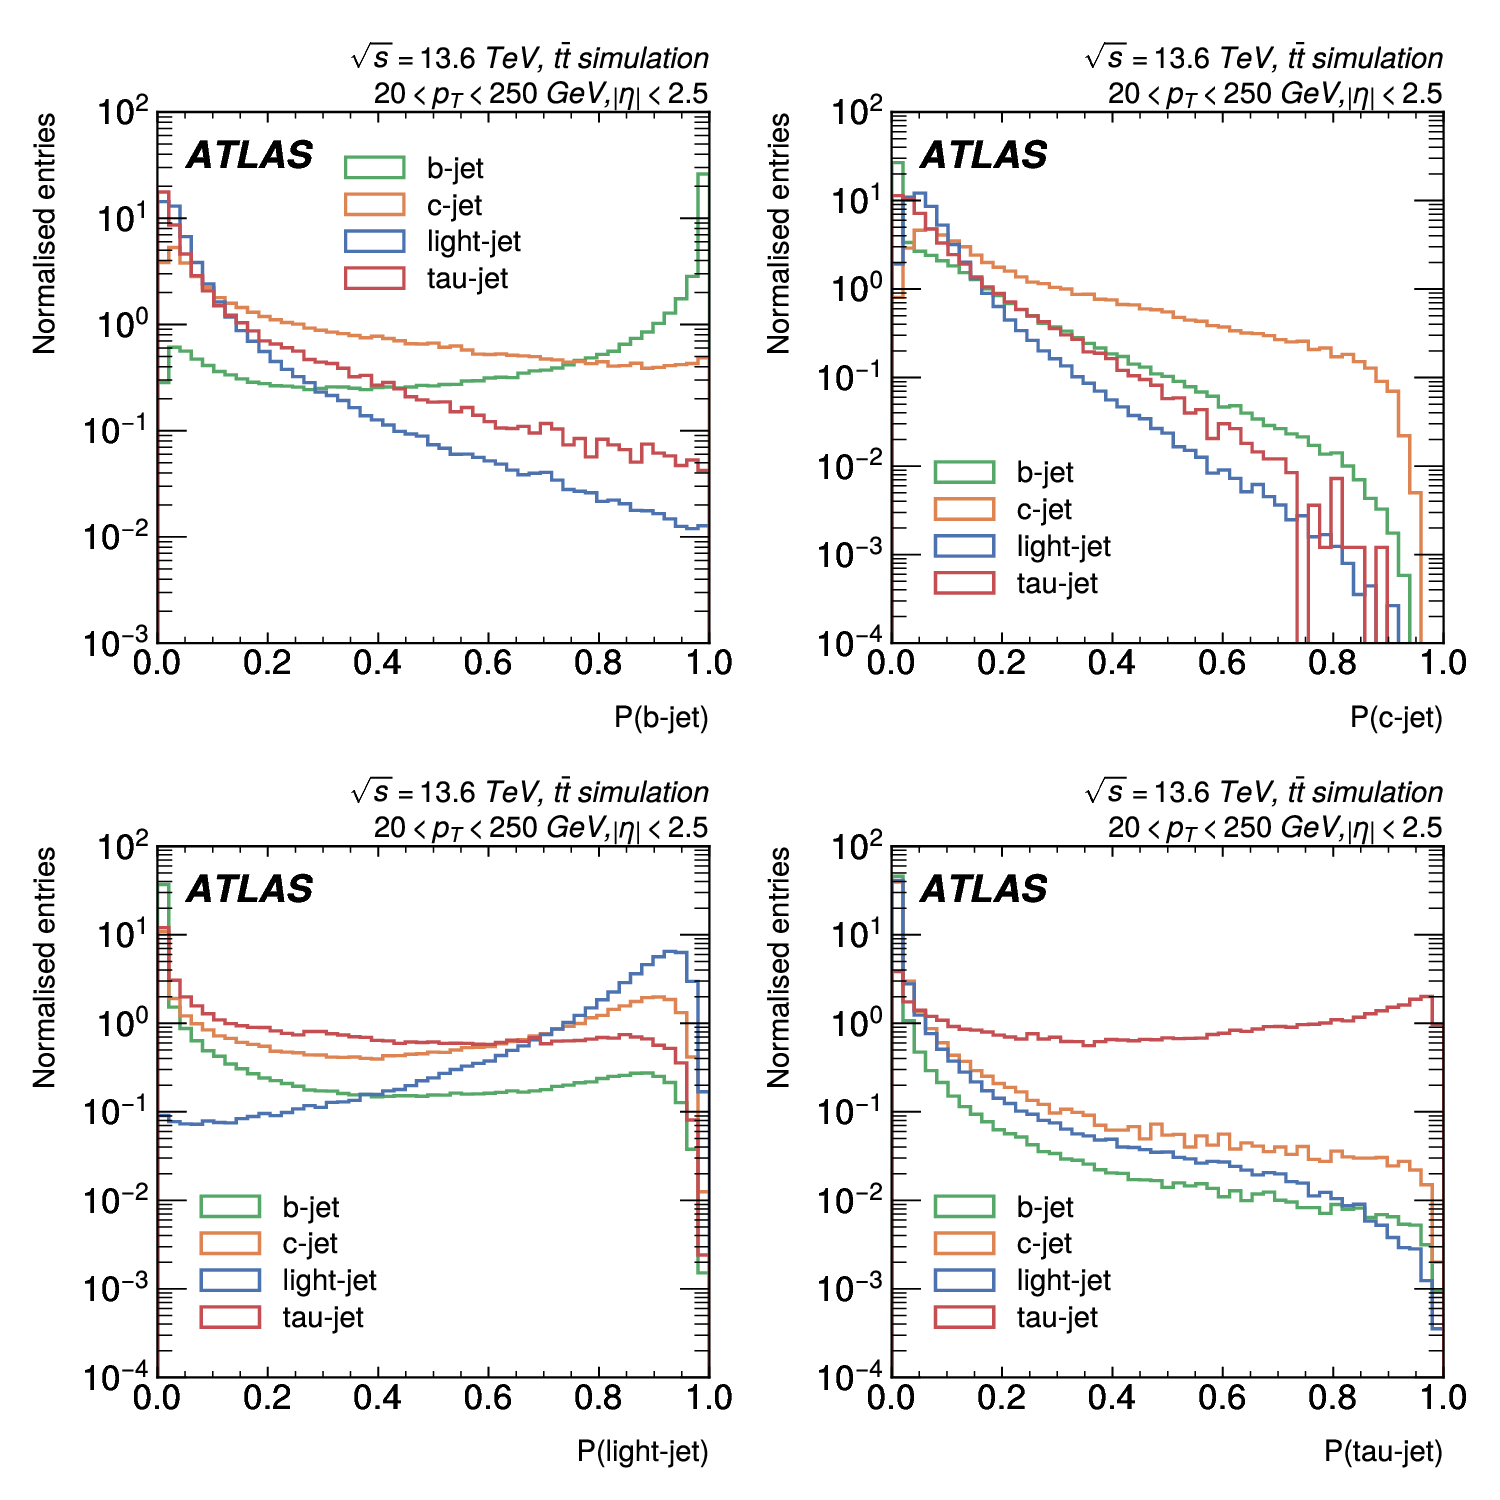
\includegraphics[width=0.82\linewidth]{../../results/eval/score_distributions.png}
                    \caption{Score softmax $P(\text{classe})$}
                \end{figure}
            \end{center}
        \end{column}
        \begin{column}{0.46\textwidth}
            \begin{center}
                \begin{figure}
                    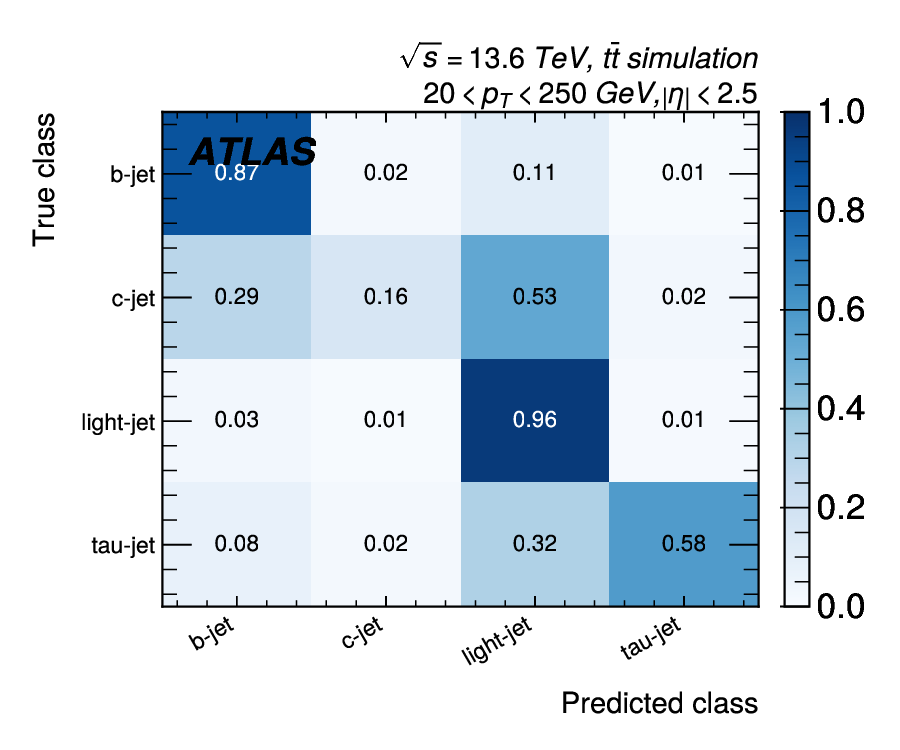
\includegraphics[width=0.82\linewidth]{../../results/eval/confusion_matrix.png}
                    \caption{Matrice di confusione (normalizzata)}
                \end{figure}
            \end{center}
        \end{column}
    \end{columns}
\end{frame}


\begin{frame}{Metriche di Classificazione e risultati ROC}
    \begin{columns}[T]
        \begin{column}{0.46\textwidth}
            \begin{block}{Metriche sul test set}
                \centering\vspace{2pt}
                \begin{tabular}{lcccc}
                    \toprule
                    Classe       & P    & R    & F1   & Acc. glob. \\
                    \midrule
                    $b$-jet      & 0.88 & 0.86 & 0.88 & \multirow{4}{*}{0.84} \\
                    $c$-jet      & 0.54 & 0.16 & 0.24 & \\
                    light-jet    & 0.83 & 0.96 & 0.89 & \\
                    $\tau$-jet   & 0.69 & 0.58 & 0.63 & \\
                    \bottomrule
                \end{tabular}
                \vspace{2pt}
            \end{block}
            \begin{block}{Cause del basso F1 sui $c$-jet}
                Dataset fortemente sbilanciato: $c$-jet e $\tau$-jet sottorappresentati
            \end{block}
        \end{column}
        \begin{column}{0.50\textwidth}
            \begin{block}{Rigetto del fondo al 70\% di eff.\ $b$-tagging}
                \centering\vspace{2pt}
                \begin{tabular}{lcc}
                    \toprule
                    Fondo       & GN2 (ATLAS) & Questa impl. \\
                    \midrule
                    Jet-$c$     & 50          & 12  \\
                    Jet leggero & 2000        & 700 \\
                    Jet-$\tau$  & 400         & 100 \\
                    \bottomrule
                \end{tabular}
                \vspace{6pt}
            \end{block}
            \begin{block}{Rigetto del fondo al 30\% di eff.\ $c$-tagging}
                \centering\vspace{2pt}
                \begin{tabular}{lcc}
                    \toprule
                    Fondo       & GN2 (ATLAS) & Questa impl. \\
                    \midrule
                    Jet-$b$     & 20          & 12  \\
                    Jet leggero & 300         & 70  \\
                    Jet-$\tau$  & 60          & 4   \\
                    \bottomrule
                \end{tabular}
                \vspace{2pt}
            \end{block}
        \end{column}
    \end{columns}
\end{frame}


\begin{frame}{Curve ROC: risultati e confronto ($b$-tagging)}
    \begin{columns}[T]
        \begin{column}{0.53\textwidth}
            \begin{center}
                \begin{figure}
                    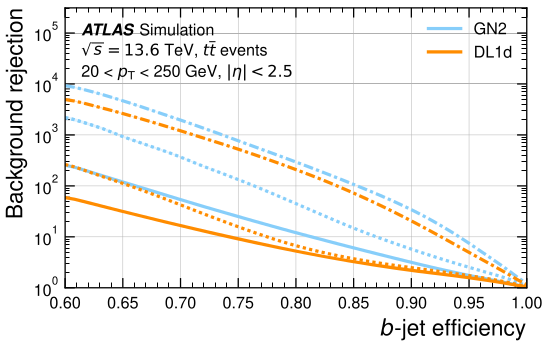
\includegraphics[width=0.82\linewidth]{../../results/article_b_jet.png}
                \end{figure}
            \end{center}
        \end{column}
        \begin{column}{0.45\textwidth}
            \begin{center}
                \begin{figure}
                    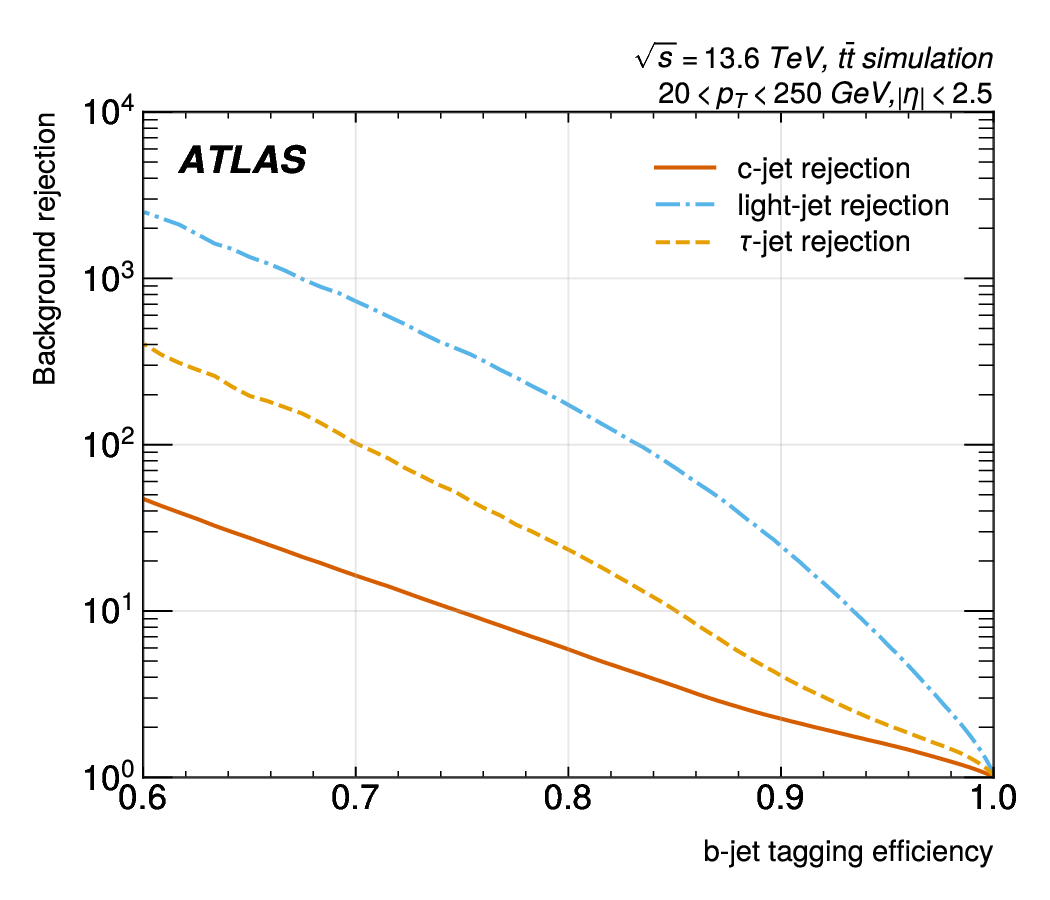
\includegraphics[width=0.82\linewidth]{../../results/eval/roc_db.png}
                \end{figure}
            \end{center}
        \end{column}
    \end{columns}
    \begin{alertblock}{Interpretazione}
        Le discrepanze sono ragionevoli con l'architettura ridotta ($\sim$230\,000 vs. milioni di parametri GN2), il dataset più piccolo e l'assenza di ottimizzazione sistematica degli iperparametri
    \end{alertblock}
\end{frame}


\begin{frame}{Curve ROC: risultati e confronto ($c$-tagging)}
    \begin{columns}[T]
        \begin{column}{0.53\textwidth}
            \begin{center}
                \begin{figure}
                    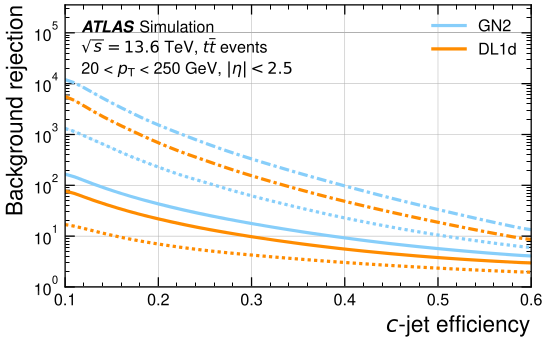
\includegraphics[width=0.82\linewidth]{../../results/article_c_jet.png}
                \end{figure}
            \end{center}
        \end{column}
        \begin{column}{0.45\textwidth}
            \begin{center}
                \begin{figure}
                    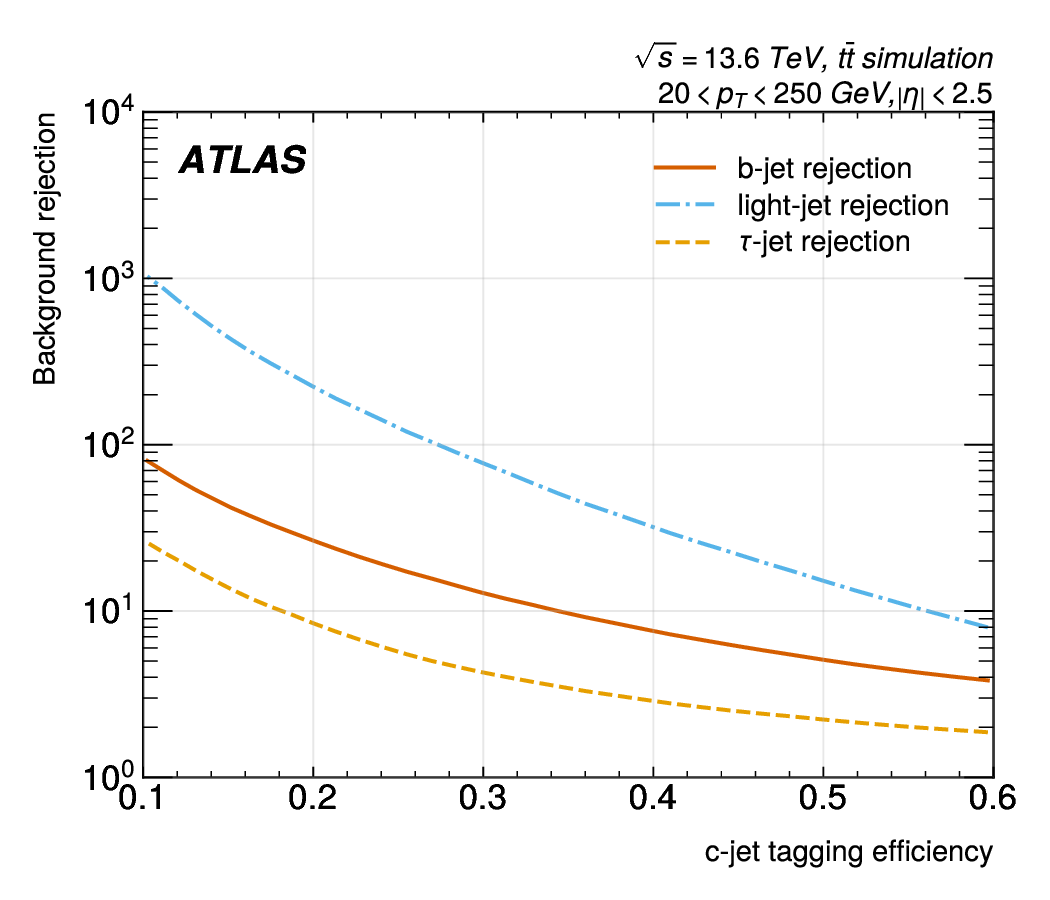
\includegraphics[width=0.82\linewidth]{../../results/eval/roc_dc.png}
                \end{figure}
            \end{center}
        \end{column}
    \end{columns}
    \begin{alertblock}{Interpretazione}
        Le discrepanze sono ragionevoli con l'architettura ridotta ($\sim$230\,000 vs. milioni di parametri GN2), il dataset più piccolo e l'assenza di ottimizzazione sistematica degli iperparametri
    \end{alertblock}
\end{frame}


\begin{frame}{Sommario e Sviluppi Futuri}
    \begin{columns}[T]
        \begin{column}{0.48\textwidth}
            \begin{block}{Cosa è stato implementato}
                \begin{itemize}
                    \item[$\checkmark$] Pipeline completa: \texttt{preprocess} $\to$ \texttt{dataset} $\to$ \texttt{train} $\to$ \texttt{evaluate}
                    \item[$\checkmark$] Architettura GN2 + ottimizzazione I/O
                \end{itemize}
            \end{block}
            \begin{block}{Sviluppi futuri}
                \begin{itemize}
                    \item Obiettivi ausiliari (origine tracce + vertici)
                    \item Ottimizzazione degli iperparametri
                    \item Training su dataset completo
                \end{itemize}
            \end{block}
        \end{column}
        \begin{column}{0.48\textwidth}
            \begin{block}{Risultati principali}
                Il modello riproduce \textbf{qualitativamente} il comportamento atteso:
                \begin{itemize}
                    \item Buona separazione dei $b$-jet e light-jet
                    \item Difficoltà strutturale su $c$-jet e $\tau$-jet
                \end{itemize}
                Prestazioni quantitative inferiori a GN2 di un fattore $\sim 3-4$ ($b$-tagging) e $\sim 5-10$ ($c$-tagging)
            \end{block}
        \end{column}
    \end{columns}
    \vspace{4pt}
    \begin{alertblock}{Limitazione principale}
        I due \textbf{obiettivi di addestramento ausiliari} (classificazione dell'origine delle tracce e raggruppamento per vertice comune) potrebbero contribuire fino al 30\% di miglioramento nel rigetto del fondo
    \end{alertblock}
\end{frame}


\begin{frame}{Appendice: distribuzione jet flavour}
    \begin{center}
        \begin{figure}
            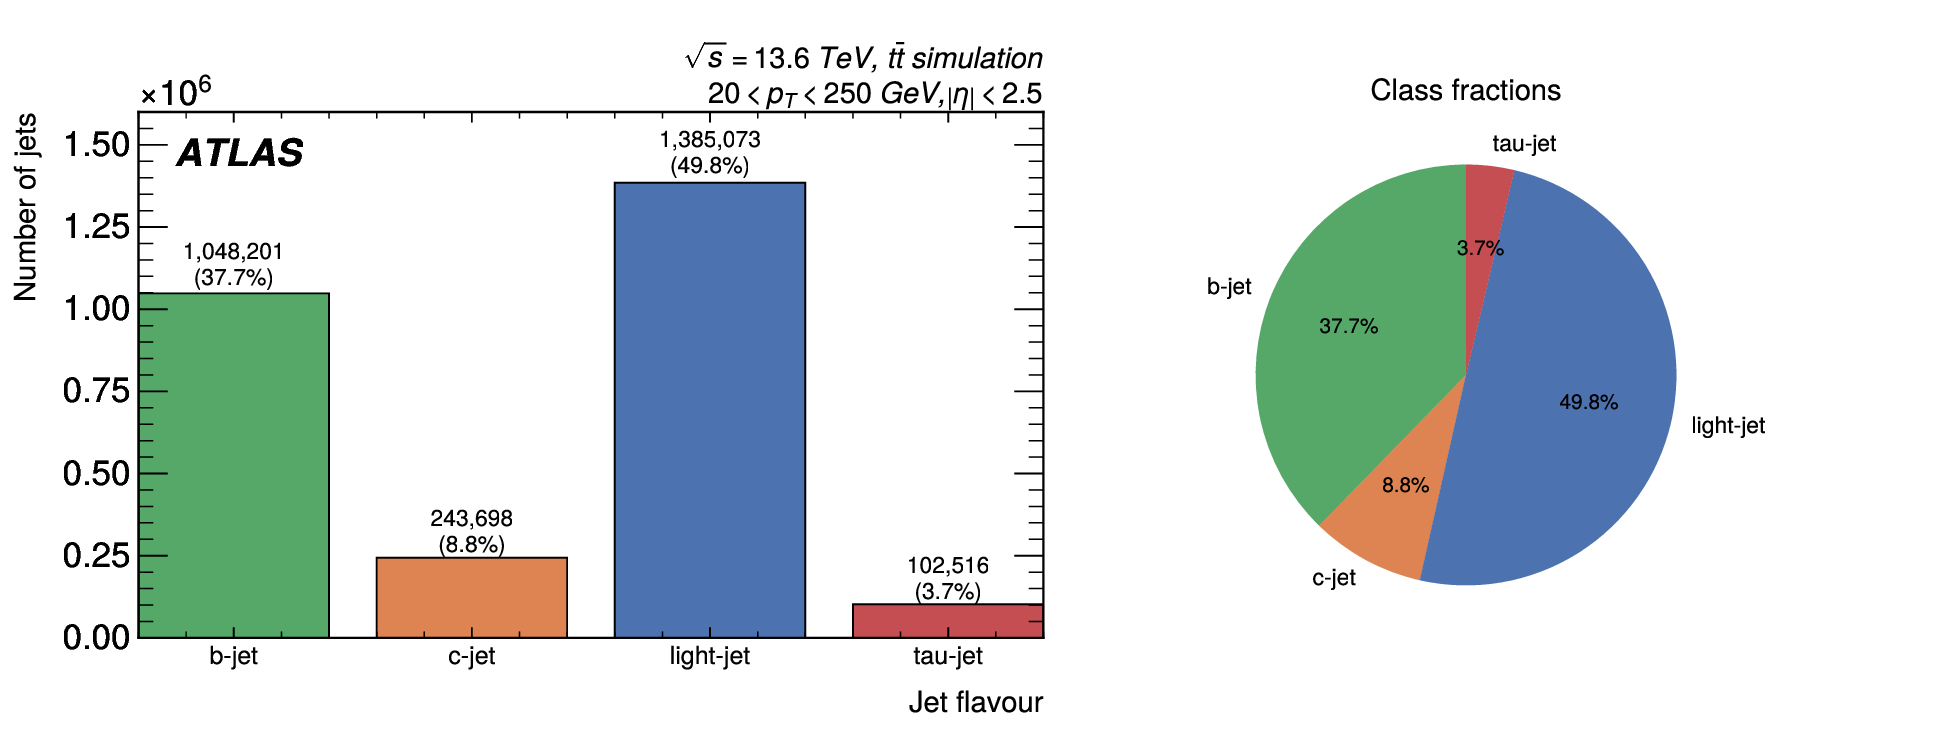
\includegraphics[width=0.95\linewidth]{../../results/data_statistics/label_distribution.png}
        \end{figure}
    \end{center}
\end{frame}


\begin{frame}{Appendice: correlazioni tra feature}
    \begin{columns}[T]
        \begin{column}{0.43\textwidth}
            \begin{center}
                \begin{figure}
                    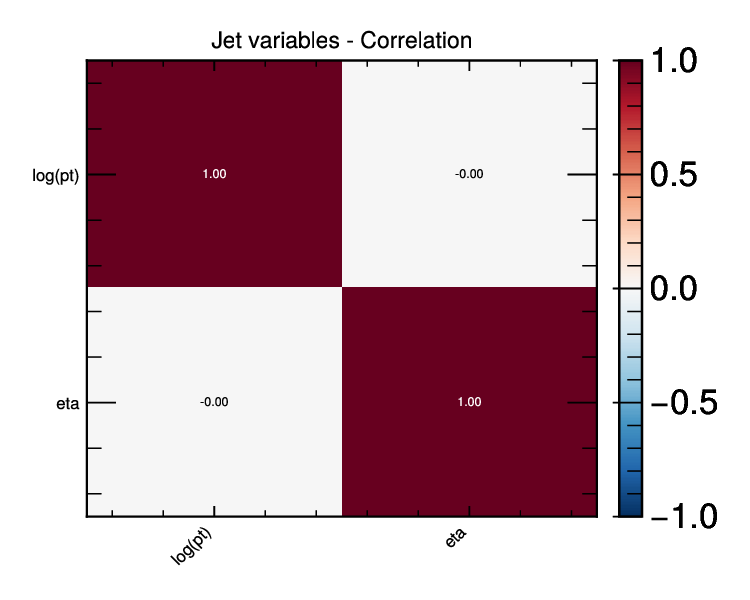
\includegraphics[width=0.82\linewidth]{../../results/data_statistics/correlation_jet.png}
                \end{figure}
            \end{center}
        \end{column}
        \begin{column}{0.55\textwidth}
            \begin{center}
                \begin{figure}
                    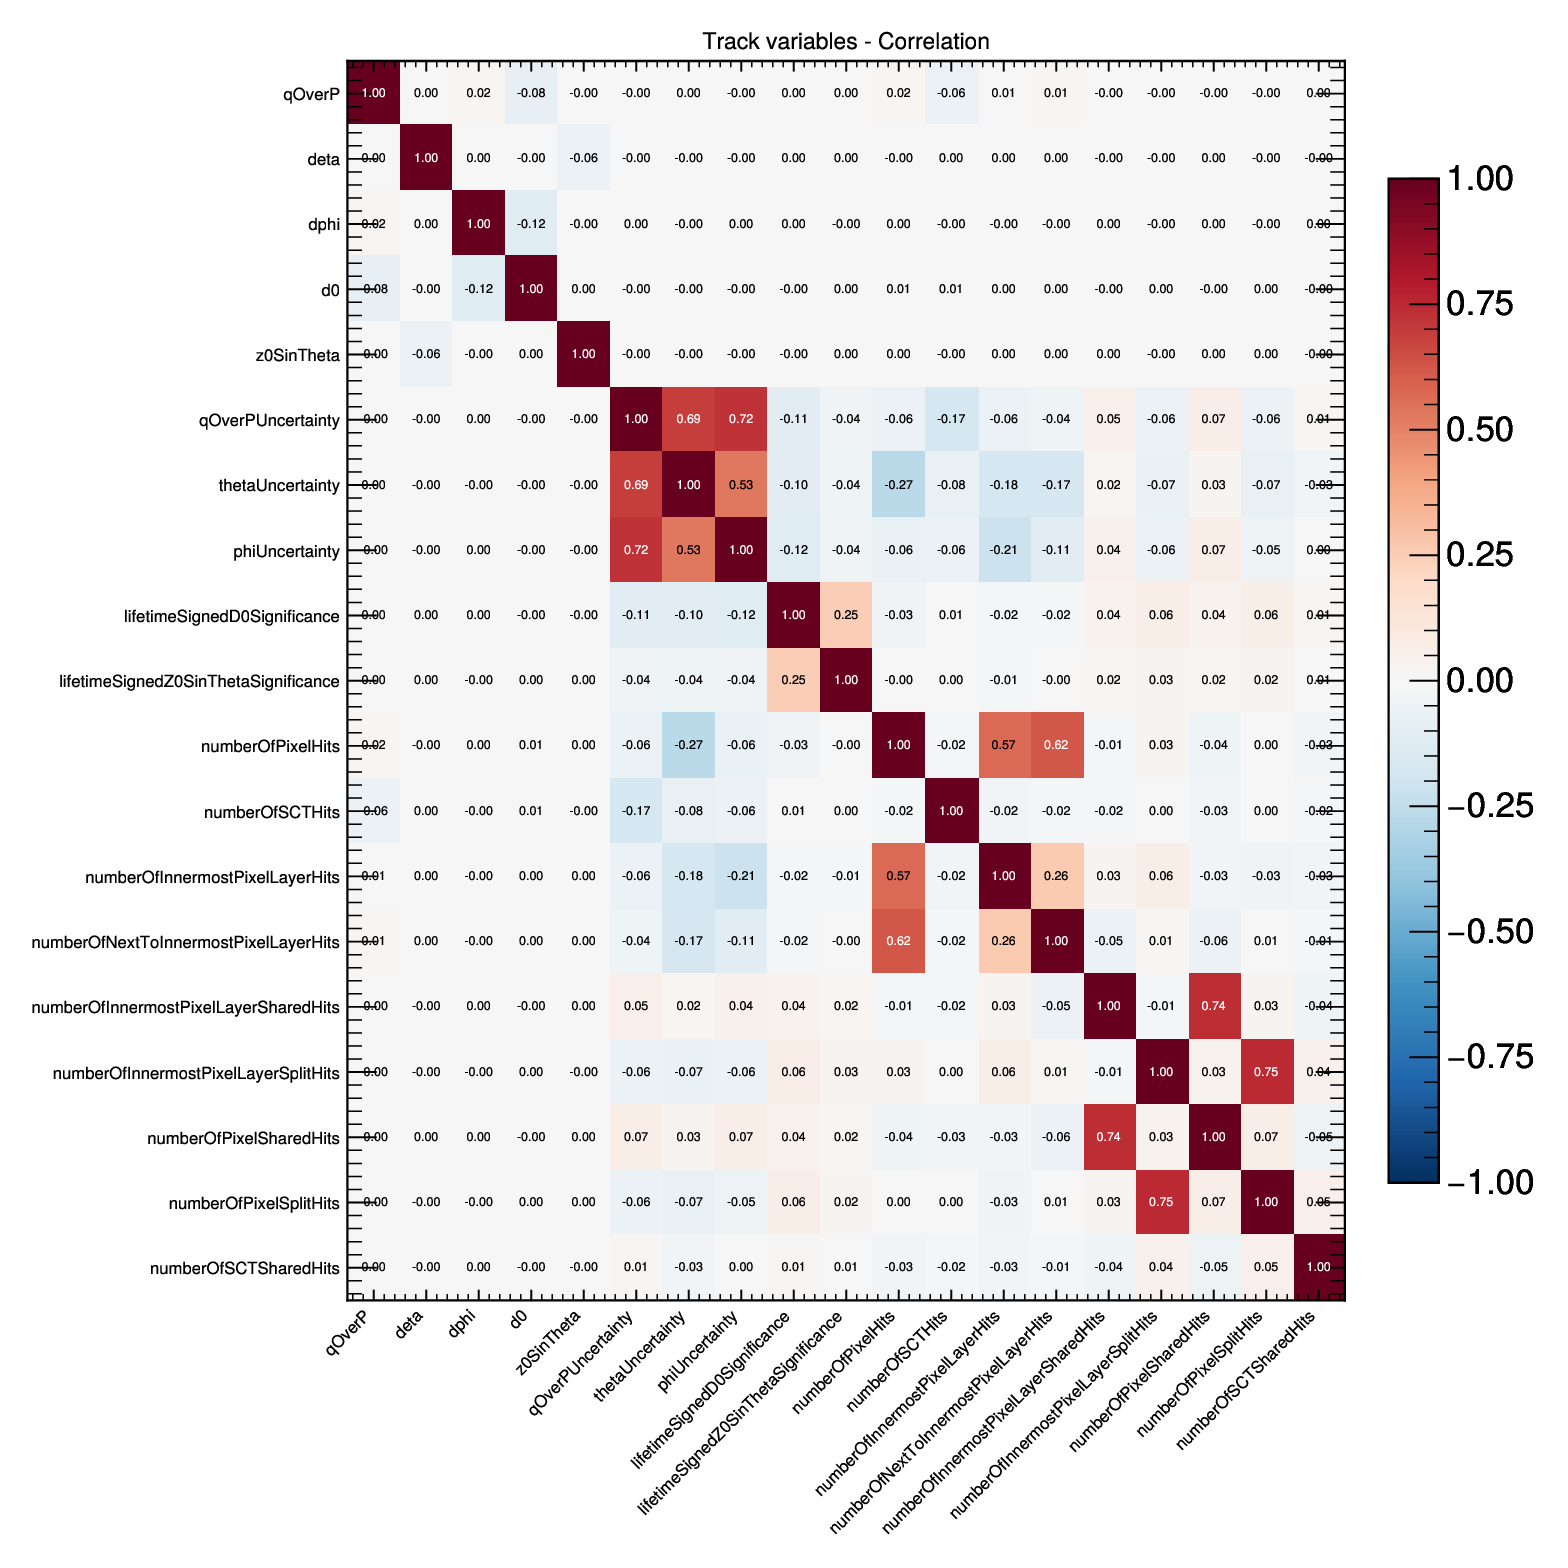
\includegraphics[width=0.82\linewidth]{../../results/data_statistics/correlation_track.png}
                \end{figure}
            \end{center}
        \end{column}
    \end{columns}
\end{frame}


\begin{frame}{Appendice: discriminanti}
    \begin{columns}[T]
        \begin{column}{0.49\textwidth}
            \begin{center}
                \begin{figure}
                    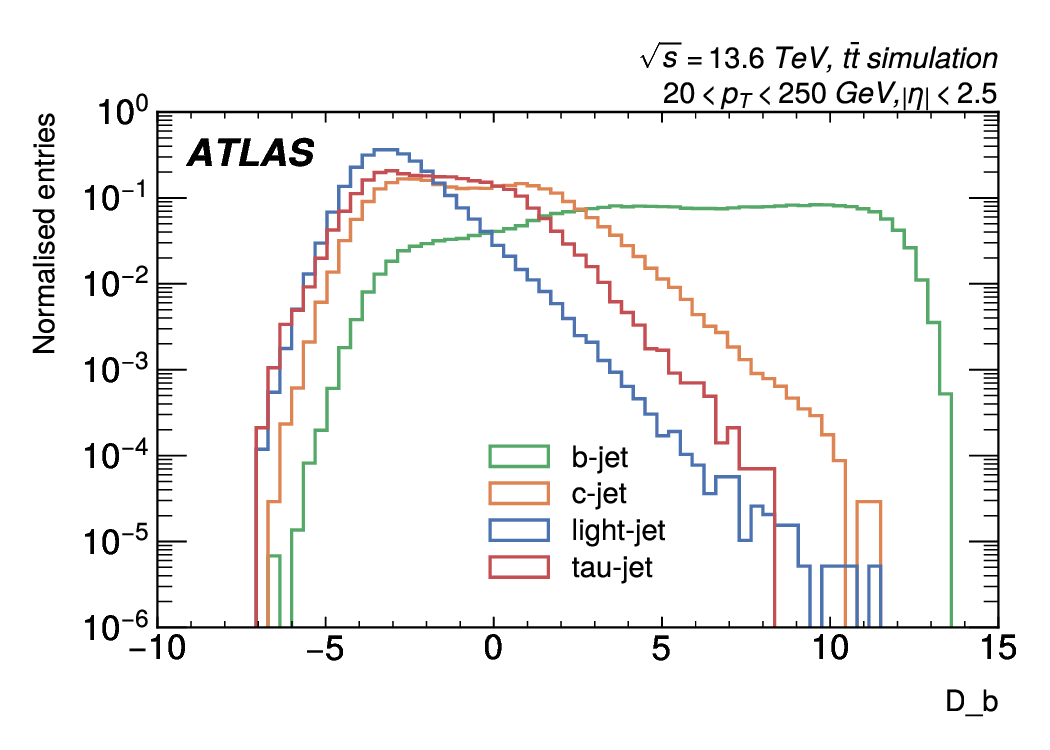
\includegraphics[width=0.95\linewidth]{../../results/eval/discriminant_db.png}
                \end{figure}
            \end{center}
        \end{column}
        \begin{column}{0.49\textwidth}
            \begin{center}
                \begin{figure}
                    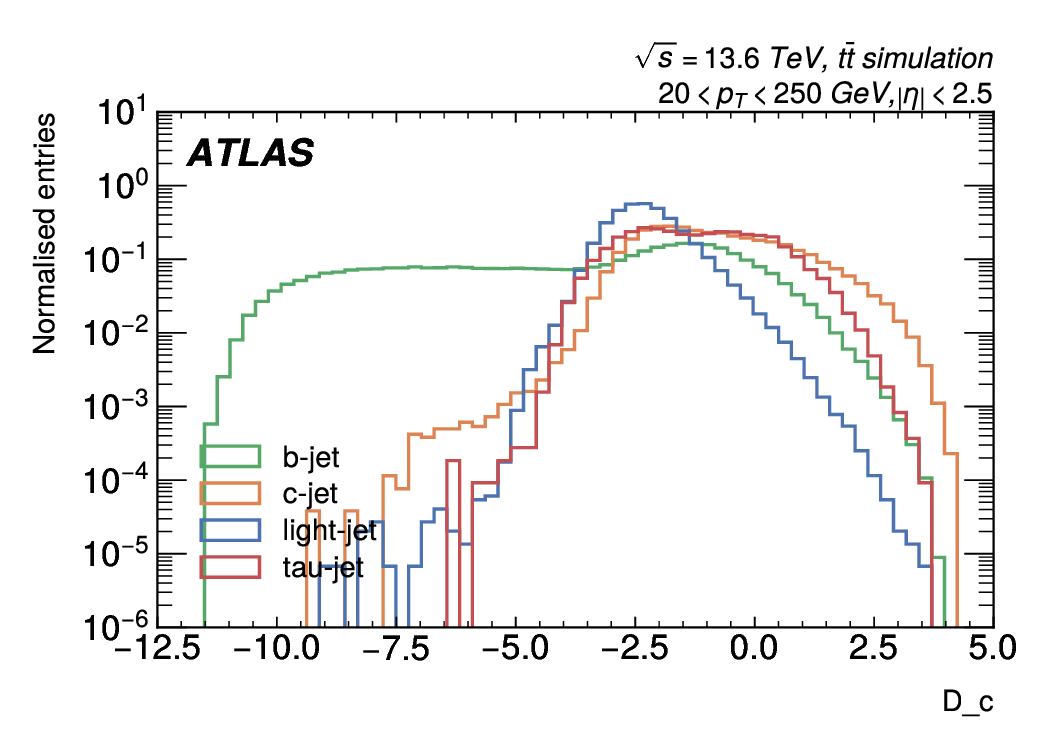
\includegraphics[width=0.95\linewidth]{../../results/eval/discriminant_dc.png}
                \end{figure}
            \end{center}
        \end{column}
    \end{columns}
\end{frame}

\end{document}